\documentclass[t, screen, aspectratio=43]{beamer}
\usepackage[T1]{fontenc}
\usepackage[utf8]{inputenc}
\usepackage{epsf}
\usepackage{graphicx}
\usepackage{geometry}
\usepackage{tabularx}
\usepackage[table]{colortbl}
\usepackage{xcolor}
\usepackage{soul}
\usepackage[normalem]{ulem}
\usepackage{tikz}
\usepackage{subcaption}
% Use the NTNU-temaet for beamer 
% \usetheme[style=ntnu|simple|vertical|horizontal, 
%     language=bm|nn|en, 
%     smalltitle, 
%     city=all|trondheim|alesund|gjovik]{ntnu2017}
\usetheme[style=helvet,language=en]{ntnu2017}

\usepackage[english]{babel}
\usepackage[style=numeric,backend=biber,natbib=false,sorting=none]{biblatex}

\title[Short title]{Python Framework for Design and Analysis of Integer-N ADPLLs}
\subtitle{Specialization Project Progress - 12th Week}
\author[C Nielsen]{Cole Nielsen}
\institute[NTNU]{Department of Electronic Systems, NTNU}
\date{15 November 2019 (Calendar week 46)}
%\date{} % To have an empty date

\addbibresource{example.bib} % Add bibliography database

% Set the reference style to numeric.
% See here: http://tex.stackexchange.com/questions/68080/beamer-bibliography-icon
\setbeamertemplate{bibliography item}[text] 

% Set bibliography fonts to a small size.
\renewcommand*{\bibfont}{\footnotesize}




\begin{document}

\begin{frame}
	\titlepage%
\end{frame}

% Alternatively, special title page command to get a different background
% \ntnutitlepage

% #############################################################################
% Timeline
% #############################################################################

\begin{frame}
	\frametitle{Timeline}
	\begin{table}[htb!]
		\tiny
		\centering
		\vspace{-1em}
		\def\arraystretch{1.5}		
		\setlength\arrayrulewidth{0.75pt}
		\setlength{\tabcolsep}{1em} % for the horizontal padding
		\begin{tabular}{|l|l|l|l|}
			\hline 
			\rule[-1ex]{0pt}{2.5ex} \cellcolor{gray!40}\textbf{Week} & \cellcolor{gray!40}\textbf{Dates} &\cellcolor{gray!40}\textbf{Tasks} & \cellcolor{gray!40}\textbf{Outcomes}\\ 
			\hline 
			\rule[-1ex]{0pt}{2.5ex} \cellcolor{red!20}\textbf{36}& \cellcolor{red!20}2.9 - 8.9 & \cellcolor{red!20}Review PLL Design & \cellcolor{red!20}Refreshed Knowledge\\ 
			\hline 
			\rule[-1ex]{0pt}{2.5ex} \cellcolor{red!20}\textbf{37}& \cellcolor{red!20}9.9 - 15.9 & \cellcolor{red!20}Modeling/simulation (set up) & \cellcolor{red!20}--\\ 
			\hline 
			\rule[-1ex]{0pt}{2.5ex} \cellcolor{red!20}\textbf{38}& \cellcolor{red!20}16.9 - 22.9 & \cellcolor{red!20}Modeling/simulation &\cellcolor{red!20}TDC/DCO Requirements\\ 
			\hline 
			\rule[-1ex]{0pt}{2.5ex} \cellcolor{red!20}\textbf{39}& \cellcolor{red!20}23.9 - 29.9& \cellcolor{red!20}Modeling/simulation& \cellcolor{red!20}Loop Filter/Digital Algorithms\\ 
			\hline 
			\rule[-1ex]{0pt}{2.5ex} \cellcolor{red!20}\textbf{40}& \cellcolor{red!20}30.9 - 6.10& \cellcolor{red!20}Modeling/simulation& \cellcolor{red!20}{Loop filter, DCO, TDC, calibration}\color{black}\\ 
			\hline 
			\rule[-1ex]{0pt}{2.5ex} \cellcolor{red!20}\textbf{41}&\cellcolor{red!20}7.10 - 13.10&\cellcolor{red!20}Circuit Research &\cellcolor{red!20}DCO/Divider topologies\\ 
			\hline 
			\rule[-1ex]{0pt}{2.5ex} \cellcolor{red!20}\textbf{42}&\cellcolor{red!20}14.10 - 20.10&\cellcolor{red!20}Circuit Research &\cellcolor{red!20}TDC/other topologies\\ 
			\hline 
			\rule[-1ex]{0pt}{2.5ex} \cellcolor{red!20}\textbf{43}&\cellcolor{red!20}21.10 - 27.10&\cellcolor{red!20}Spur analysis, filter automation &\cellcolor{red!20} \\ 
			\hline 
			\rule[-1ex]{0pt}{2.5ex} \cellcolor{red!20}\textbf{44}&\cellcolor{red!20}28.10 - 3.11&\cellcolor{red!20}Filter automation, SNR estimation&\cellcolor{red!20}\\ 
			\hline 
			\rule[-1ex]{0pt}{2.5ex} \cellcolor{red!20}\textbf{45}&\cellcolor{red!20}4.11 - 10.11&\cellcolor{red!20}Variation analysis, flicker noise &\cellcolor{red!20}Histograms/yield estimates\\ 
			\hline 
			\rule[-1ex]{0pt}{2.5ex} \cellcolor{green!20}\textbf{46}&\cellcolor{green!20}11.11 - 17.11&\cellcolor{green!20}Real DCO sensitivity, TDC/divider jitter&\cellcolor{green!20}Simlate ring-DCO in Virtuoso\\ 
			\hline 
			\rule[-1ex]{0pt}{2.5ex} \textbf{47}& 18.11 - 24.11& PLL + Radio simulation& BER estimate\\ 
			\hline 
			\rule[-1ex]{0pt}{2.5ex} \textbf{48}& 25.11 - 1.12& Agglomerate into cohesive framework & (I have an Exam on 30.11)\\ 
			\hline 
			\rule[-1ex]{0pt}{2.5ex} \textbf{49}& 2.12 - 8.12& Finish framework, report writing& \\ 
			\hline 
			\rule[-1ex]{0pt}{2.5ex} \textbf{50}& 9.12 - 15.12& Report writing& Complete before 15.12\\ 
			\hline 
		\end{tabular}
		\begin{flushleft}\textbf{Legend:} \colorbox{red!20}{\textbf{Done}} \colorbox{green!20}{\textbf{Current}}  \colorbox{blue!20}{\textbf{Revised}}
		% *I will write the report simultaneously with the work.
		\end{flushleft}
		% \caption{Assigned specifications for branch line hybrid design.}
		% \label{asgn_specs}
	\end{table}   
\end{frame}


% #############################################################################
% This week
% #############################################################################

\begin{frame}
	\frametitle{Timeline Tasks}
	\begin{block}{This week}
		\begin{itemize}
			\footnotesize
			\item \textbf{Include more sources of phase noise in PLL model:}
			\begin{itemize}
				\footnotesize
				\item Added divider jitter, LF quantization noise, DCO quantization noise.
			\end{itemize} 
			\item \textbf{Simulation of Ring oscillator in 22FDX:}
			\begin{itemize}
				\footnotesize
				\item Extracted values/variation for $V_{th}$ and body effect coefficient $\gamma$ for RVT/SLVT devices in various conditions.
				\item Extracted data for frequency and current consumption for varied L, (W/L), load capacitance, temperature, supply voltage and RVT/SLVT devices.
				\item Simulated variance of ring oscillator for comparison to model.
			\end{itemize} 
		\end{itemize}    
	\end{block}
\end{frame}

% #############################################################################
% sim/modeling approach
% #############################################################################

\begin{frame}
	\frametitle{Phase noise model}
	\begin{block}{Adding more components}
			%\center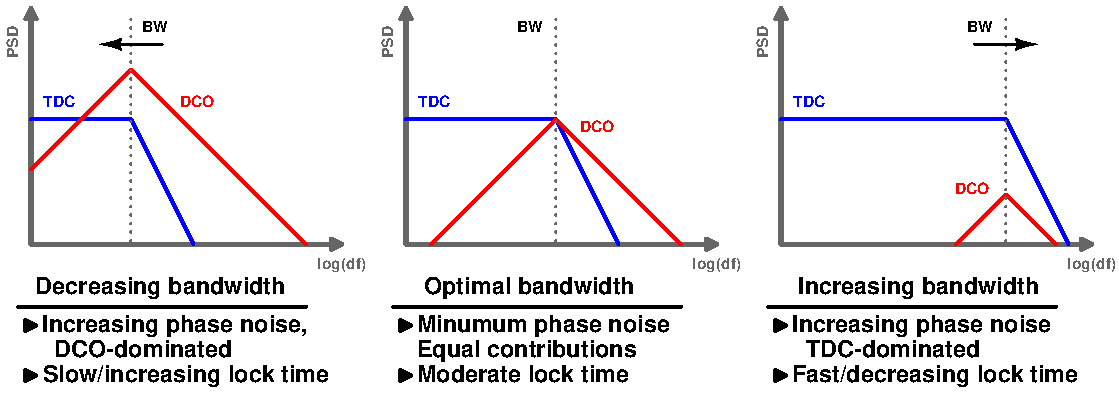
\includegraphics[width=0.8\textwidth, angle=0]{loop_bandwidth.pdf}
		\begin{itemize}
			\scriptsize
			\item New loop filter optimizer is based on phase noise minimization, it is good to have a more complete phase noise model.
			\begin{itemize}
				\scriptsize
				\item Previously only TDC noise and DCO noise (non-quantization) were considered.
			\end{itemize}
			\item New phase noise components that were added:
			\begin{itemize}
				\scriptsize
				\item Loop filter quantization noise.
				\item DCO quantization noise
				\item Divider jitter.
			\end{itemize}
			\item These added components will allow for a more accurate estimate of the oscillator phase noise, and thus better loop filter optimization (i.e. phase noise minimizaton).
		\end{itemize}    
	\end{block}
\end{frame}

\begin{frame}
	\frametitle{Phase noise model}
	\begin{block}{Adding more components}
			%\center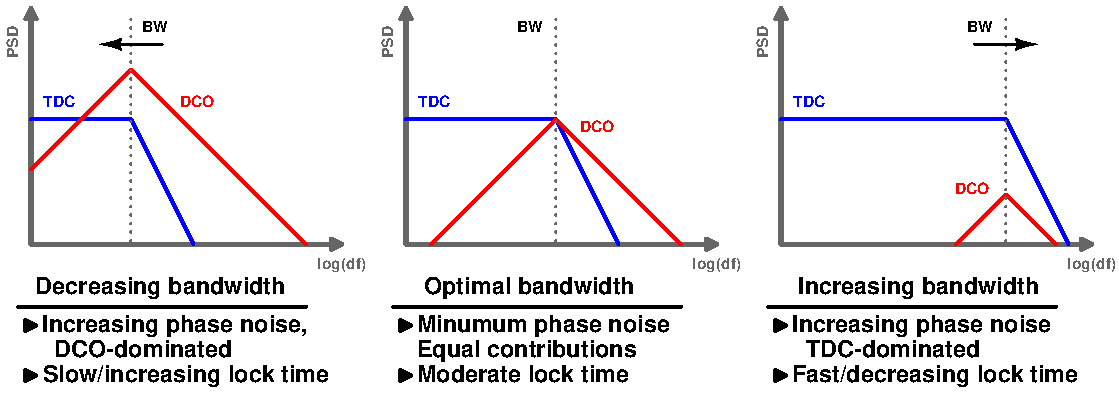
\includegraphics[width=0.8\textwidth, angle=0]{loop_bandwidth.pdf}
		\begin{itemize}
			\scriptsize
			\item \textbf{Loop filter/DCO quantization noise}, where $Q_{DCO}$ and $Q_{LF}$ are the DCO and loop filter quantization noise signals. The noise transfer function is:
			\begin{equation}
				\frac{\Phi_{out}}{Q_{DCO}} = \frac{\Phi_{out}}{Q_{LF}} = 2\pi\frac{N_{DIV}}{M_{TDC}}\frac{G(s)}{H_{LF}(s)}
			\end{equation}
			The PLL output phase noise spectral density from DCO quantization is as follows:
			\begin{equation}
				S_{\Phi_{out} Q_{DCO}} = \frac{1}{12f_{clk}}\left|2\pi\frac{N_{DIV}}{M_{TDC}}\frac{G(s)}{H_{LF}(s)}\right|^2
			\end{equation}	
			The PLL output phase noise spectral density from loop filter quantization is as follows, where $\sigma_{Q_{LF}}^2$ is average power (in LSB$^2$) of the quantization noise. This is implementation dependent.
			\begin{equation}
				S_{\Phi_{out} Q_{LF}} = \sigma_{Q_{LF}}^2\left|2\pi\frac{N_{DIV}}{M_{TDC}}\frac{G(s)}{H_{LF}(s)}\right|^2
			\end{equation}			
		\end{itemize}    
	\end{block}
\end{frame}

\begin{frame}
	\frametitle{Phase noise model}
	\begin{block}{Adding more components}
			%\center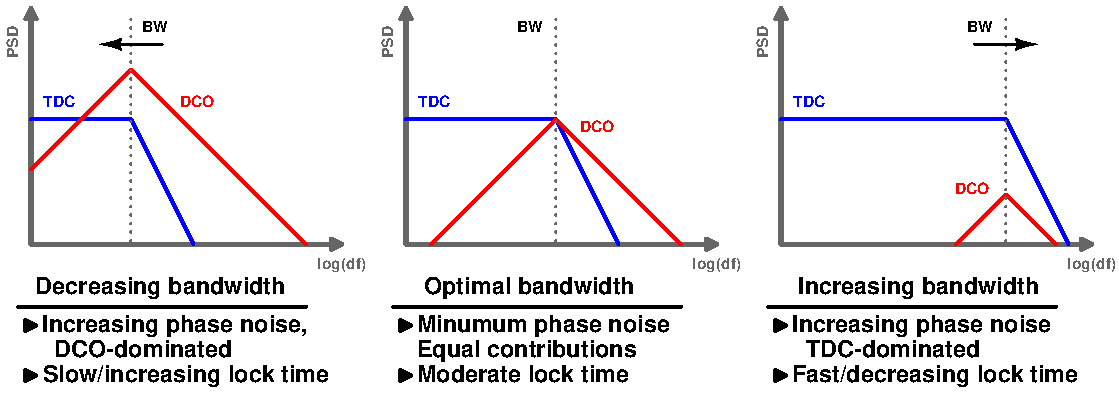
\includegraphics[width=0.8\textwidth, angle=0]{loop_bandwidth.pdf}
		\begin{itemize}
			\scriptsize
			\item \textbf{Divider jitter}, where the noise transfer function is:
			\begin{equation}
				\frac{\Phi_{out}}{\Phi_{div}} = -N\cdot G(s)
			\end{equation}
			If the divider is subject to jitter in time with variance $\sigma_{jit,div}^2$, the corresponding PLL output phase noise spectrum is:
			\begin{equation}
				S_{\Phi_{out} \Phi_{jit,div}} = \left|2\pi f_{clk} N_{DIV} \sigma_{jit,div}G(s)\right|^2
			\end{equation}	
			This has the same dependence on G(s) as TDC quantization noise. To make divider noise less than TDC-related noise, we set $S_{\Phi_{out} \Phi_{jit,div}} < S_{\Phi_{out} \Phi_{Q_{TDC}}}$, this results in:
			\begin{equation}
				\sigma_{jit,div} < \frac{1}{M\cdot f_{clk}^{3/2}}
			\end{equation}
		\end{itemize}    
	\end{block}
\end{frame}

\begin{frame}
	\frametitle{Ring oscillator in 22FDX}
	\begin{block}{Extracting FET parameters}
			%\center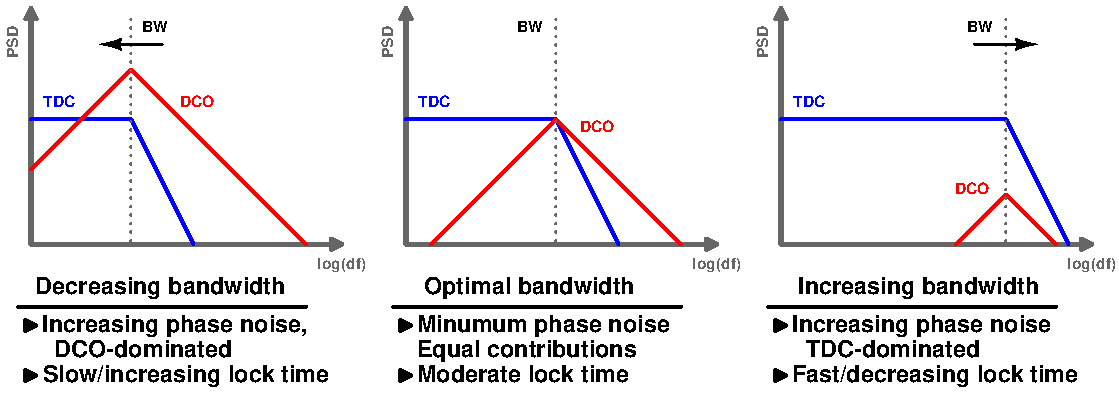
\includegraphics[width=0.8\textwidth, angle=0]{loop_bandwidth.pdf}
		\begin{itemize}
			\scriptsize
			\item Extracted $V_{th}$ and body effect coefficient to use with model for comparison with simulation.
			\item Extracted for RVT and SLVT devices with L in \{20n 100n, 500n\}, W/L in \{1, 10\}.
			\item Short channel effects noticable in 20nm, $>=$ 100 nm it becomes less significant. 
			\item For L=500nm, the below parameters were found. $\sigma_{V_{th}} < 0.036 V_{th}$, $\sigma_{\gamma} < 0.024 \gamma$ (via Monte Carlo samping at T=-40, 25, 85).
		\end{itemize}    
		\begin{table}[htb!]
			\tiny
			\centering
			\def\arraystretch{1.5}		
			\setlength\arrayrulewidth{0.75pt}
			\setlength{\tabcolsep}{1em} % for the horizontal padding
			\begin{tabular}{|l|l|l|l|l|}
				\hline 
				\rule[-1ex]{0pt}{2.5ex} \cellcolor{gray!40}\textbf{Parameter} & \cellcolor{gray!40}\textbf{NFET} & \cellcolor{gray!40}\textbf{SLVTNFET}& \cellcolor{gray!40}\textbf{PFET} & \cellcolor{gray!40}\textbf{SLVTPFET} \\ 
				\hline 
				\rule[-1ex]{0pt}{2.5ex} $V_{th}$ [mV] & 390-0.69T & 340-0.67T & -387+0.88T & -312+0.77T\\ 
				\hline 
				\rule[-1ex]{0pt}{2.5ex} $\gamma $ [V/V]  & -0.072 & -0.083 & 0.082 & 0.069\\ 
				\hline 
			\end{tabular} 
			% \caption{Assigned specifications for branch line hybrid design.}
			% \label{asgn_specs}
		\end{table}   
	\end{block}
\end{frame}

\begin{frame}
	\frametitle{Ring oscillator in 22FDX}
	\begin{block}{Ring oscillator model - assumptions}
			%\center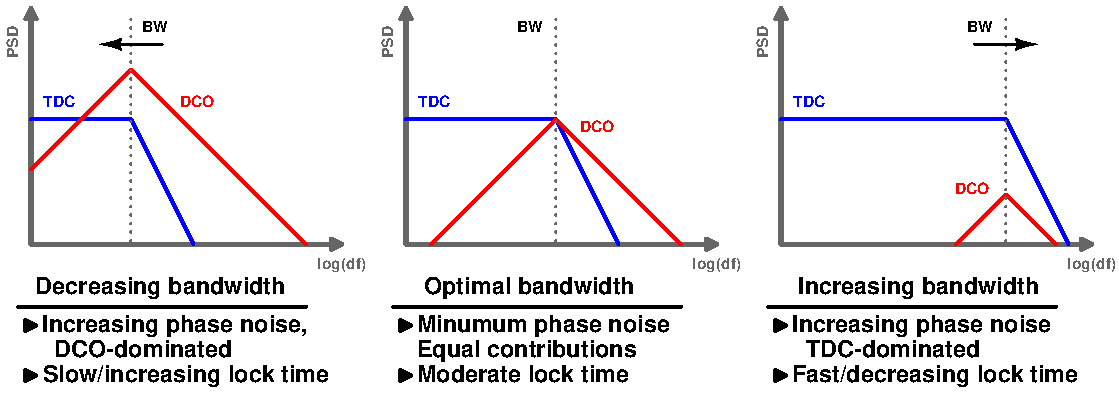
\includegraphics[width=0.8\textwidth, angle=0]{loop_bandwidth.pdf}
		\begin{itemize}
			\scriptsize
			\item Model ring oscillator with inverters modeled with ideal switches and lumped R and C components. The R is equivalent to the average channel resistance for the FETs.
			\item Square law ($L>>L_{min}$) and in saturation during period of propagtion delay. Requires 0.25$V_{DD}$ < $V_{th}$ < 0.5$V_{DD}$.
		\end{itemize}    
		\center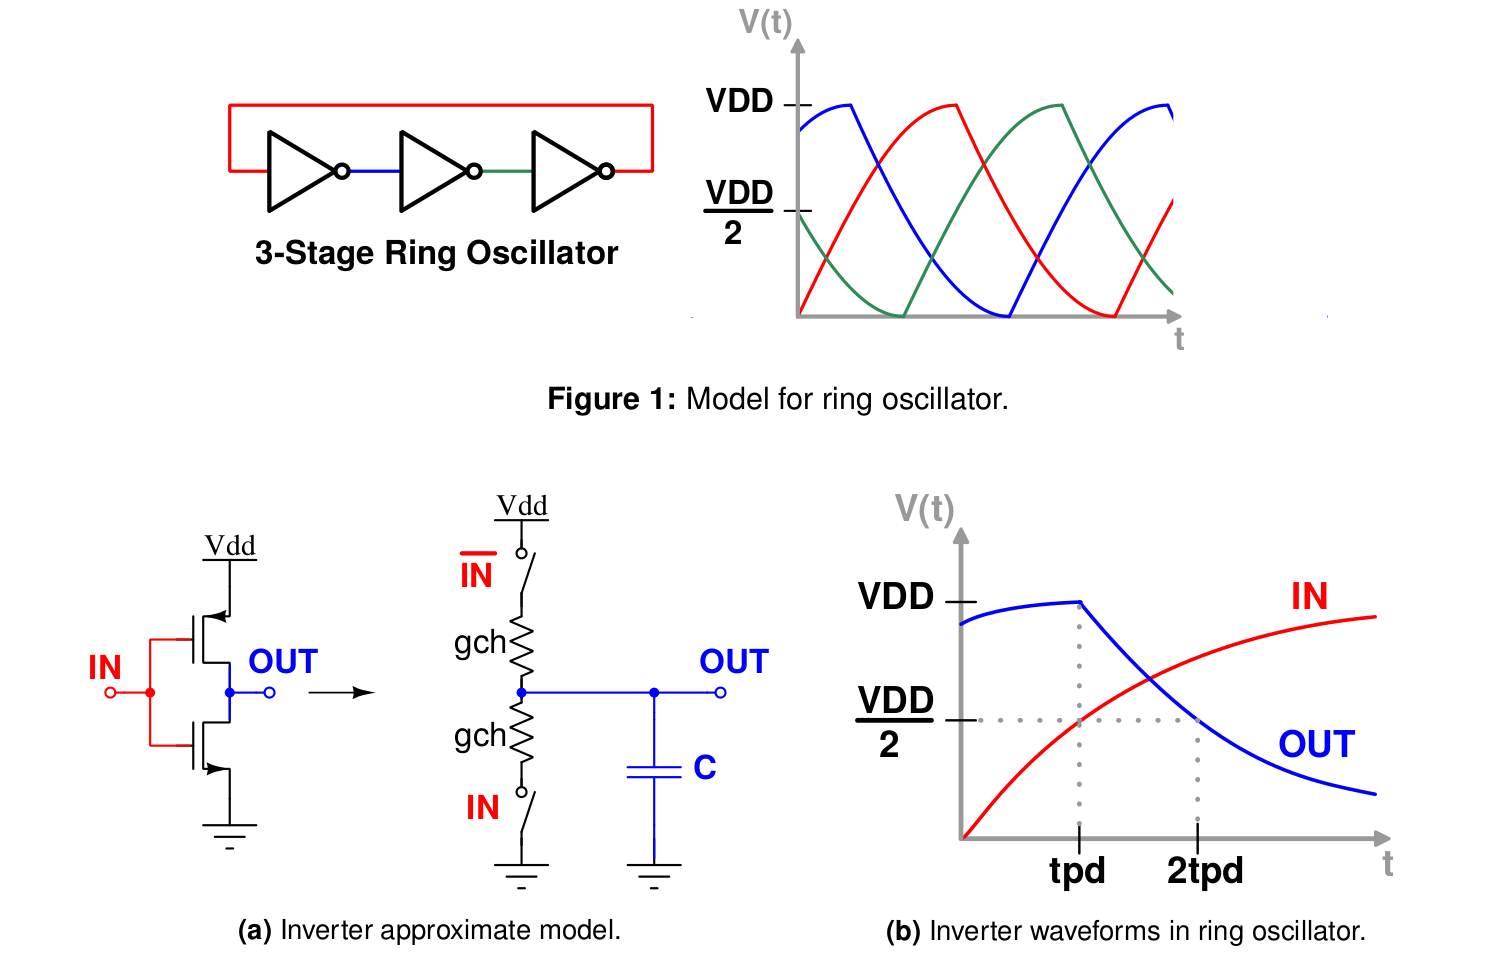
\includegraphics[width=0.5\linewidth]{ro_model_fig.png}
	\end{block}
\end{frame}


\begin{frame}
	\frametitle{Ring oscillator in 22FDX}
	\begin{block}{Ring oscillator model - equations}
			%\center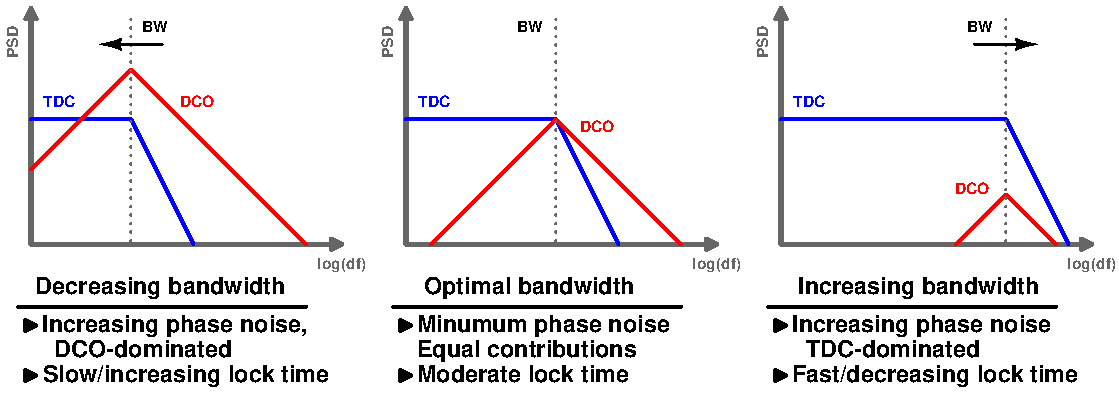
\includegraphics[width=0.8\textwidth, angle=0]{loop_bandwidth.pdf}
	\scriptsize
	\vspace{-1em}
	\begin{equation}
		f_{osc} = \frac{\mu_nC_{ox}}{4\ln2NC}\left(\frac{W}{L}\right)_n\left[V_{DD}\left(\frac{7}{8\ln2}-1\right)-V_{t0}\left(\frac{1}{\ln2}-1\right) + \gamma V_{BG}\left(\frac{1}{\ln2}-1\right) \right]
	\end{equation}
	\begin{equation}
		\Delta f_{osc}(V_{BG}) = \gamma V_{BG}\frac{\mu_nC_{ox}}{4\ln2NC}\left(\frac{W}{L}\right)_n\left[\frac{1}{\ln2}-1\right]
	\end{equation}	
	If backgate voltage is limited to the range of $V_{DD}$
	\begin{equation}
		f_{c} = \frac{\mu_nC_{ox}}{4\ln2NC}\left(\frac{W}{L}\right)_n\left[V_{DD}\left(\frac{7}{8\ln2}-1+\frac{\gamma}{2\ln2}-\frac{\gamma}{2}\right)-V_{t0}\left(\frac{1}{\ln2}-1\right)\right]
	\end{equation}
	\begin{equation}
		\Delta f = \frac{\gamma V_{DD}}{2}\frac{\mu_nC_{ox}}{4\ln2NC}\left(\frac{W}{L}\right)_n\left[\frac{1}{\ln2}-1\right]
	\end{equation}
	\begin{equation}
		\frac{\Delta f}{f_c} = \frac{1}{2}\cdot\frac{\gamma V_{DD}\left( 1-\ln2 \right)}{V_{DD}\left(\frac{7}{8}-\ln2+\frac{\gamma}{2}-\frac{\gamma}{2}\ln2\right)-V_{t0}\left(1-\ln2\right)}
	\end{equation}	  
	\end{block}
\end{frame}

\begin{frame}
	\frametitle{Ring oscillator in 22FDX}
	\begin{block}{Ring oscillator simulation - schematic}
			%\center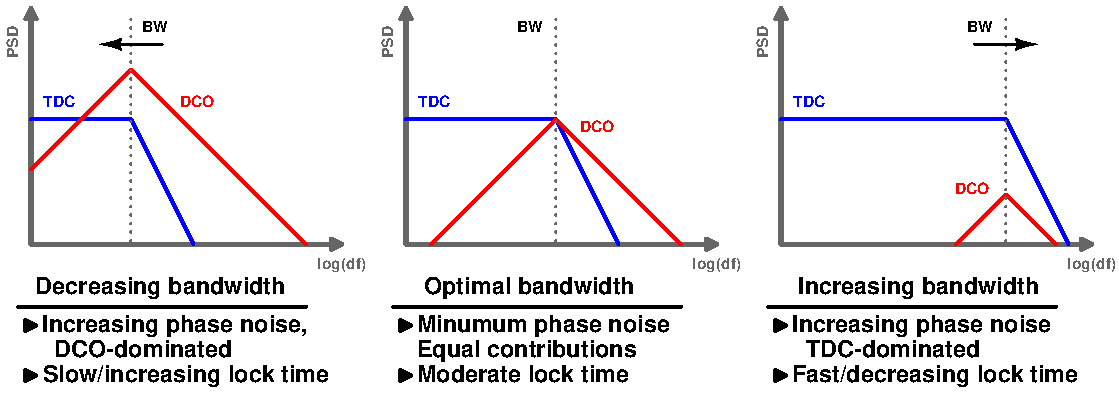
\includegraphics[width=0.8\textwidth, angle=0]{loop_bandwidth.pdf}
		\begin{itemize}
			\scriptsize
			\item Simulated simple 5 stage ring oscillator with $V_{DD}$ = 0.8.
			\item Used RVT/SLVT devices, varied temp in \{-40, 25, 85\}, L in \{100n, 500n\}, W/L in \{1, 10\}, $C_{load}$ in \{0, 1f, 10f\}, $V_{BB}$ in \{0, 0.8\}
		\end{itemize}    
		\center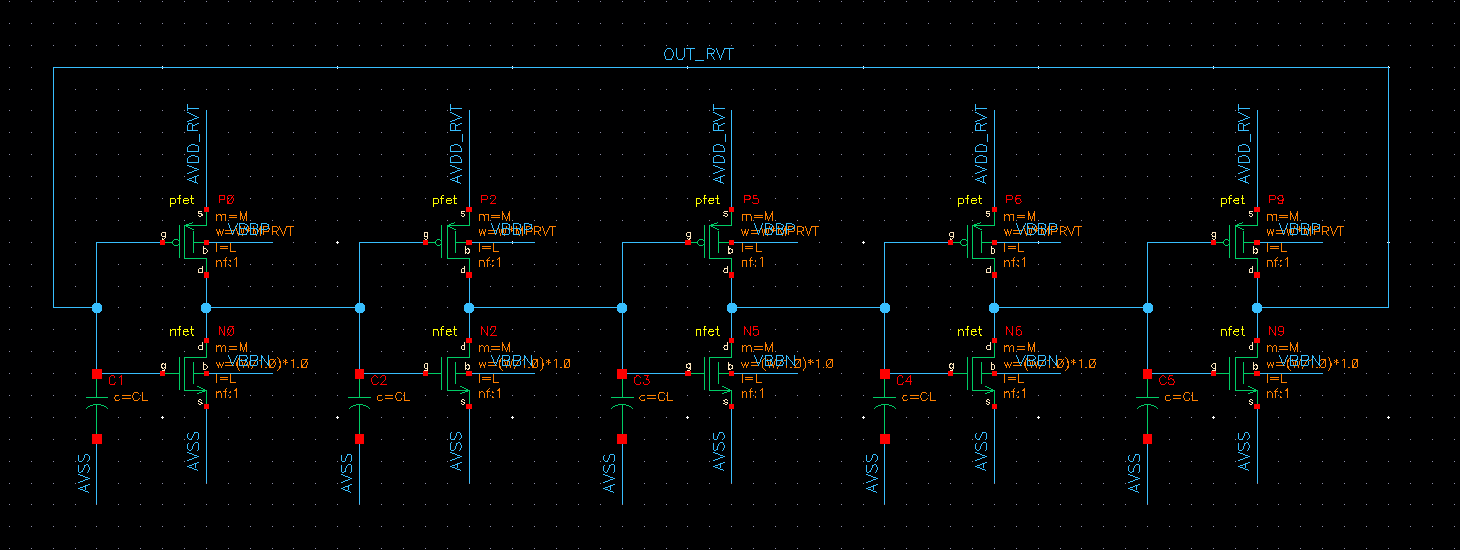
\includegraphics[width=0.8\linewidth]{ro_schem.png}
	\end{block}
\end{frame}

\begin{frame}
	\frametitle{Ring oscillator in 22FDX}
	\begin{block}{Ring oscillator simulation - variation}
			%\center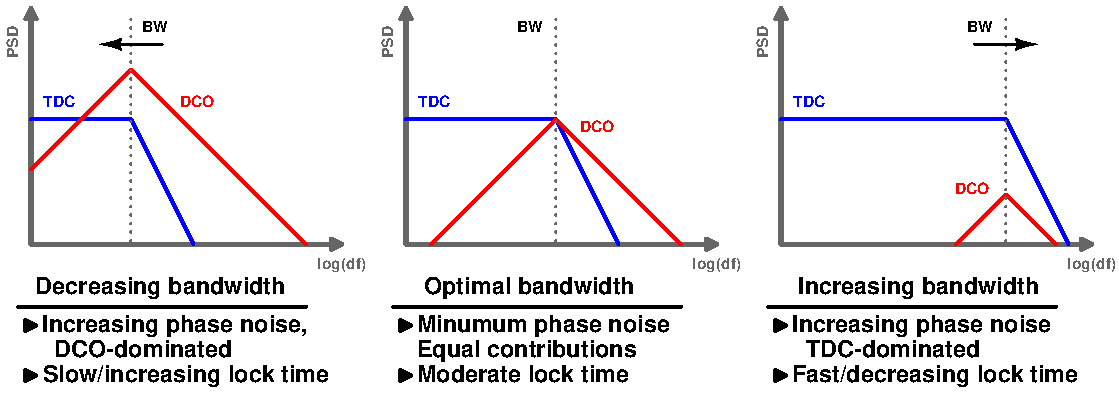
\includegraphics[width=0.8\textwidth, angle=0]{loop_bandwidth.pdf}
		\begin{itemize}
			\scriptsize
			\item Simulated simple 5 stage ring oscillator with $V_{DD}$ = 0.8.
			\item Used RVT/SLVT devices, varied temp in \{-40, 25, 85\}, L in \{100n, 500n\}, W/L in: \{1, 10\}, $C_{load}$ in \{0, 1f, 10f\}, $V_{BB}$ in \{0, 0.8\}
			\item Also perfomed Monte-Carlo at 25C with L=500nm and W/L=1:
			\item Standard deviation for RVT is 4.7\% of nominal value, for SLVT it is 4.5\% of nominal.
		\end{itemize}    
		\center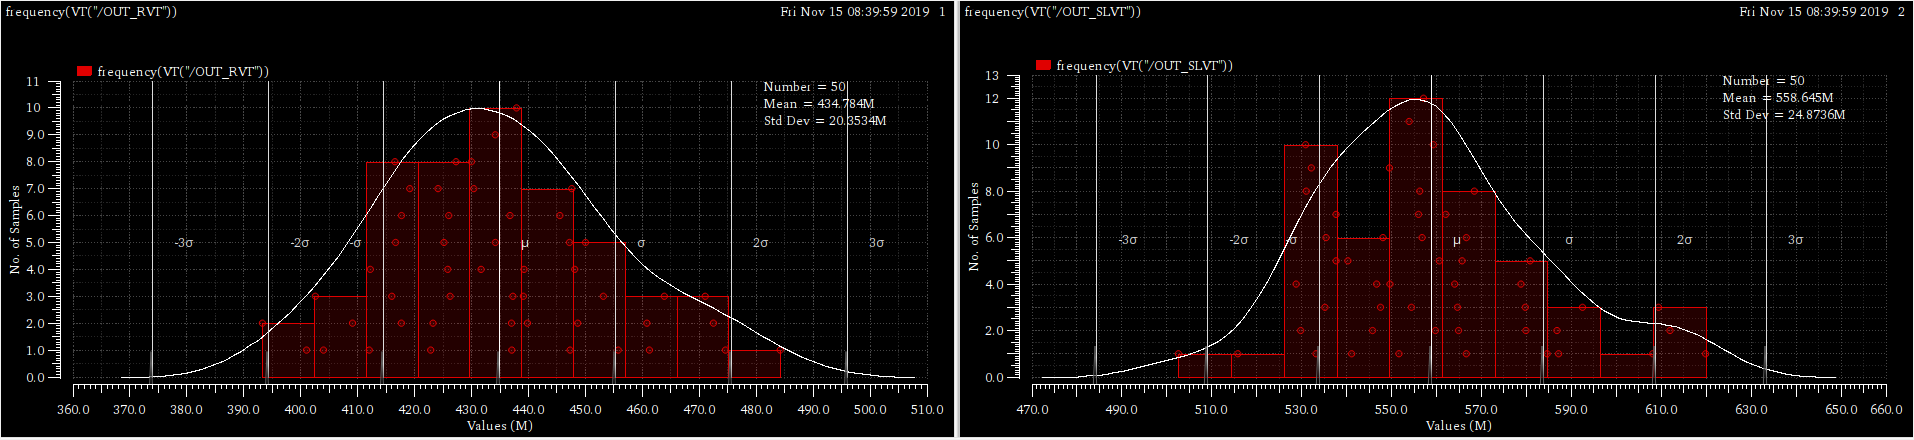
\includegraphics[width=0.8\linewidth]{freq_var.png}
	\end{block}
\end{frame}






% #############################################################################
% Loop Dynamics (continuous)
% #############################################################################

% \begin{frame}
% 	\frametitle{Loop Dynamics}
% 	\begin{block}{Still To Do}
% 		\vspace{-.2em}
% 		\begin{itemize}
% 			\footnotesize
% 			\item Standard approach to used mixed continuous/discrete time mathematical model for DPLL. 
% 			\item Plot of RO phase noise (typical)
% 			\item Automatic analysis of performance (lock detection, residual phase modulation, lock-in/pull-in range).
% 			\item Automatic optimization (using gradient descent) of PLL parameters?
% 			\item Z-domain modeling of loop? Develop (by hand) some ideal transfer funtions for loop.

% 		\end{itemize}    
% 	\end{block}
% \end{frame}

% #############################################################################
% Specification
% #############################################################################

\begin{frame}
	\frametitle{Specification (unchanged)\color{black}}
	\begin{block}{System Performance Targets}
		\scriptsize
		\begin{table}[h!]
			\centering
			\def\arraystretch{1.5}		
			\setlength\arrayrulewidth{0.75pt}
			\setlength{\tabcolsep}{1em} % for the horizontal padding
			\begin{tabular}{|l|r|l|l|}
				\hline 
				\rule[-1ex]{0pt}{2.5ex} \cellcolor{gray!40}\textbf{Parameter} & \cellcolor{gray!40}\textbf{Value} & \cellcolor{gray!40}\textbf{Unit }& \cellcolor{gray!40}\textbf{Notes}\\ 
				\hline 
				\rule[-1ex]{0pt}{2.5ex} \textbf{Frequency}  & 2.4-2.4835 & GHz & 2.4G ISM Band\\ 
				\hline 
				\rule[-1ex]{0pt}{2.5ex} \textbf{Ref. frequency} & 16 & MHz & Yields 6 channels \\ 
				\hline 
				\rule[-1ex]{0pt}{2.5ex} \textbf{Power} & $\leq$ 100  &$\mu$W & \\ 
				\hline 
				\rule[-1ex]{0pt}{2.5ex} \textbf{FSK BER} & $\leq$ 1e-2  & & 2FSK with $f_{dev}$=$\pm$250 KHz\\ 
				\hline 
				\rule[-1ex]{0pt}{2.5ex} \textbf{Initial Lock Time} & $\leq$ 50 & $\mu$s & Upon cold start \\ 
				\hline 
				\rule[-1ex]{0pt}{2.5ex} \textbf{Re-lock Time} & $\leq$ 5 & $\mu$s & Coming out of standby \\ 
				\hline 
				\rule[-1ex]{0pt}{2.5ex} \textbf{Bandwidth} & 50 & kHz & (nominally), tunable \\ 
				\hline 
			\end{tabular} 
			% \caption{Assigned specifications for branch line hybrid design.}
			% \label{asgn_specs}
		\end{table}   
		Additionally: PLL output should support IQ sampling at LO frequency.
	\end{block}    
\end{frame}

\begin{frame}
	\frametitle{Specification (unchanged)}
	\begin{block}{PLL Component Performance Targets}
		\scriptsize
		\begin{table}[h!]
			\centering
			\def\arraystretch{1.5}		
			\setlength\arrayrulewidth{0.75pt}
			\setlength{\tabcolsep}{1em} % for the horizontal padding
			\begin{tabular}{|l|r|l|l|}
				\hline 
				\rule[-1ex]{0pt}{2.5ex} \cellcolor{gray!40}\textbf{Parameter} & \cellcolor{gray!40}\textbf{Value} & \cellcolor{gray!40}\textbf{Unit }& \cellcolor{gray!40}\textbf{Notes}\\ 
				\hline 
				\rule[-1ex]{0pt}{2.5ex} \textbf{DCO LSB Resolution}  & $\leq$ 50  & kHz & Determined from quantization noise.\\ 
				\hline 
				\rule[-1ex]{0pt}{2.5ex} \textbf{DCO DNL} & < 1 & LSB & Ensures monotonicity \\ 
				\hline 
				\rule[-1ex]{0pt}{2.5ex} \textbf{TDC Resolution} & 0.95  & ns & \\ 
				\hline 
				\rule[-1ex]{0pt}{2.5ex} \textbf{TDC Resolution (bits)} &  6 &bits & \\ 
				\hline 
			\end{tabular} 
			% \caption{Assigned specifications for branch line hybrid design.}
			% \label{asgn_specs}
		\end{table}   
	\end{block}    
\end{frame}

% #############################################################################
% Architecture - block diagram
% #############################################################################

\begin{frame}
	\frametitle{Architecture (updated)}
	\begin{block}{Block Diagram}
	\center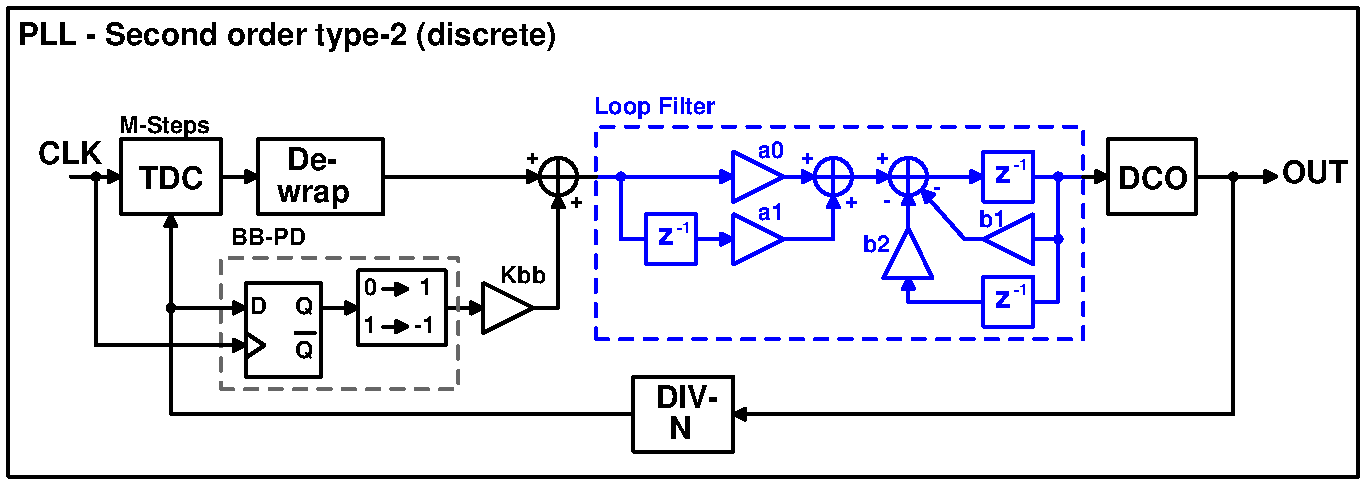
\includegraphics[width=0.8\textwidth, angle=0]{pll_sec_order_bb.pdf}

	\end{block}
		\begin{block}{Power Targets}
		\vspace{-.1em}
		\begin{table}[htb!]
			\tiny
			\centering
			\def\arraystretch{1.5}		
			\setlength\arrayrulewidth{0.75pt}
			\setlength{\tabcolsep}{1em} % for the horizontal padding
			\begin{tabular}{|l|l|l|l|l|}
				\hline 
				\rule[-1ex]{0pt}{2.5ex} \cellcolor{gray!40}\textbf{DCO} & \cellcolor{gray!40}\textbf{TDC} & \cellcolor{gray!40}\textbf{Divider }& \cellcolor{gray!40}\textbf{Other} & \cellcolor{gray!40}\textbf{SUM} \\ 
				\hline 
				\rule[-1ex]{0pt}{2.5ex} 70 $\mu$W& 20 $\mu$W & 10 $\mu$W & $<<$ 1 $\mu$W & 100 $\mu$W\\ 
				\hline 
			\end{tabular} 
			% \caption{Assigned specifications for branch line hybrid design.}
			% \label{asgn_specs}
		\end{table}   
	\end{block}

\end{frame}


% #############################################################################
% project phases
% #############################################################################


\begin{frame}
	\frametitle{Project Phases}
	\begin{block}{Autumn 2019}
		\footnotesize
		\begin{itemize}
			\item System modeling and simulation.
			\begin{itemize}
				\footnotesize
				\item Learn PLL theory in detail
				\item Evaluate feasability of PLL architectures (counter, TDC-based)
				\item Determine requirements for TDC/DCO/Divider/logic (bits of resolution, accuracy etc) to meet PLL performance specifications.
				\item Determine digital logic for loop filter, validate stability and lock time performance.
			\end{itemize}
			\item Research ultra-low power circuit topologies to implement system components that will meet determined requirements.
			\item Translate component-level specifications into schematic-level circuit designs.
			\begin{itemize}
				\footnotesize
				\item Try, fail, try again until functional at schematic level.
				\begin{itemize}
					\footnotesize
					\item I expect the TDC to be difficult.
				\end{itemize}
			\end{itemize}      
		\end{itemize}
	\end{block}
\end{frame}

% #############################################################################
% Project phases slide 2
% #############################################################################


\begin{frame}
	\frametitle{Project Phases (continued)}
	\begin{block}{Spring 2020}
		\begin{itemize}
			\footnotesize
			\item Finalize schematic-level design.
			\item Estabilish thorough tests for PLL performance (automated?) to help in layout.
			\item Layout of PLL.
			\begin{itemize}
				\footnotesize
				\item Design iteration until design specs met.
				\item Probably very time consuming.
			\end{itemize}
			\item Full characterization/validation of design performance. 
			\begin{itemize}
				\footnotesize
				\item Comprehensive Corners/Monte-Carlo testing (time consuming??)
				\item More design iteration if new issues crop up...
			\end{itemize}
			\item Thesis paper writing.
		\end{itemize}
	\end{block}
\end{frame}

% #############################################################################
% References
% #############################################################################


\begin{frame}
	\frametitle{References}
		\scriptsize
		[1] "Ultra-Low Power Wake-Up Receivers for Wireless Sensor Networks", N. Pletcher, J.M Rabaey, 2008.\\
		\hspace{16pt}\url{http://www.eecs.berkeley.edu/Pubs/TechRpts/2008/EECS-2008-59.html}\\
		\vspace{1em}
		% [2] "Minimum Achievable Phase Noise of RC Oscillators",
	% Navid et al. 2005
\end{frame}


\end{document}
